\documentclass[12pt,a4paper,oneside]{report}             % Single-side
%\documentclass[11pt,a4paper,twoside,openright]{report}  % Duplex

%\PassOptionsToPackage{chapternumber=Huordinal}{magyar.ldf}

\usepackage{fontspec}
\setmainfont{Times New Roman}  % specify a font that supports required glyphs

\usepackage{amsmath}
\usepackage{amssymb}
\usepackage[english,magyar]{babel}
\usepackage{hyperref}
\usepackage{datetime}
\usepackage{enumerate}
\usepackage[thmmarks]{ntheorem}
\usepackage{graphics}
\usepackage{epsfig}
\usepackage{listings}
\usepackage{color}
%\usepackage{fancyhdr}
\usepackage{lastpage}
\usepackage{anysize}
\usepackage{sectsty}
\usepackage{setspace}  % Ettol a tablazatok, abrak, labjegyzetek maradnak 1-es sorkozzel!
\usepackage[hang]{caption}
\usepackage{pdfpages}
\usepackage{todonotes}
\usepackage{enumitem}
\usepackage{makecell}
\usepackage[all]{nowidow}

% Use “\cite{NEEDED}” to get Wikipedia-style “citation needed” in document
\usepackage{ifthen}
\let\oldcite=\cite
\renewcommand\cite[1]{\ifthenelse{\equal{#1}{NEEDED}}{\ensuremath{^\texttt{[citation~needed]}}}{\oldcite{#1}}}

\usepackage{wrapfig}
\usepackage{float}

%--------------------------------------------------------------------------------------
% Main variables
%--------------------------------------------------------------------------------------
\newcommand{\vikszerzo}{Nyíri Tamás}
\newcommand{\vikkonzulens}{Dr.~Szeberényi Imre}
\newcommand{\vikcim}{Feladatellenőrző rendszer továbbfejlesztése}
\newcommand{\viktanszek}{Irányítástechnika és Informatika Tanszék}
\newcommand{\vikdoktipus}{Szakdolgozat}
\graphicspath{{./figures/}}

%--------------------------------------------------------------------------------------
% Page layout setup
%--------------------------------------------------------------------------------------
% we need to redefine the pagestyle plain
% another possibility is to use the body of this command without \fancypagestyle
% and use \pagestyle{fancy} but in that case the special pages
% (like the ToC, the References, and the Chapter pages)remain in plane style

\pagestyle{plain}
%\setlength{\parindent}{0pt} % áttekinthetőbb, angol nyelvű dokumentumokban jellemző
%\setlength{\parskip}{8pt plus 3pt minus 3pt} % áttekinthetőbb, angol nyelvű dokumentumokban jellemző
\setlength{\parindent}{12pt} % magyar nyelvű dokumentumokban jellemző
\setlength{\parskip}{0pt}    % magyar nyelvű dokumentumokban jellemző

\marginsize{35mm}{25mm}{15mm}{15mm} % anysize package
\setcounter{secnumdepth}{0}
\sectionfont{\large\upshape\bfseries}
\setcounter{secnumdepth}{2}
\singlespacing
\frenchspacing

%--------------------------------------------------------------------------------------
%	Setup hyperref package
%--------------------------------------------------------------------------------------
\hypersetup{
    bookmarks=true,            % show bookmarks bar?
    unicode=true,              % non-Latin characters in Acrobat’s bookmarks
    pdftitle={\vikcim},        % title
    pdfauthor={\vikszerzo},    % author
    pdfsubject={\vikdoktipus}, % subject of the document
    pdfcreator={\vikszerzo},   % creator of the document
    pdfproducer={Producer},    % producer of the document
    pdfkeywords={keywords},    % list of keywords
    pdfnewwindow=true,         % links in new window
    colorlinks=true,           % false: boxed links; true: colored links
    linkcolor=black,           % color of internal links
    citecolor=black,           % color of links to bibliography
    filecolor=black,           % color of file links
    urlcolor=black             % color of external links
}

%--------------------------------------------------------------------------------------
% Set up listings
%--------------------------------------------------------------------------------------
\lstset{
	basicstyle=\scriptsize\ttfamily, % print whole listing small
	keywordstyle=\color{black}\bfseries\underbar, % underlined bold black keywords
	identifierstyle=, 					% nothing happens
	commentstyle=\color{white}, % white comments
	stringstyle=\scriptsize\sffamily, 			% typewriter type for strings
	showstringspaces=false,     % no special string spaces
	aboveskip=3pt,
	belowskip=3pt,
	columns=fixed,
	backgroundcolor=\color{lightgray},
} 		
\def\lstlistingname{lista}	

%--------------------------------------------------------------------------------------
%	Some new commands and declarations
%--------------------------------------------------------------------------------------
\newcommand{\code}[1]{{\upshape\ttfamily\scriptsize\indent #1}}

% define references
\newcommand{\figref}[1]{\ref{figure:#1}. ábra}
\renewcommand{\eqref}[1]{(\ref{eq:#1})}
\newcommand{\listref}[1]{\ref{listing:#1}.}
\newcommand{\sectref}[1]{\ref{sect:#1}}
\newcommand{\tabref}[1]{\ref{tab:#1}.}

\newcommand{\sectsep}{
	\par \nopagebreak
	\parbox{\linewidth}{
    	\centering\bigskip$\ast\quad\ast\quad\ast$\par\bigskip
	}
}

\DeclareMathOperator*{\argmax}{arg\,max}
%\DeclareMathOperator*[1]{\floor}{arg\,max}
\DeclareMathOperator{\sign}{sgn}
\DeclareMathOperator{\rot}{rot}
\definecolor{lightgray}{rgb}{0.95,0.95,0.95}

\author{\vikszerzo}
\title{\viktitle}
\includeonly{
	1_abstract,
	declaration,
	2_introduction,
	3_jporta,
	4_dynamic,
	5_exercise,
	acknowledgement,
	bibliography,
	summary,
	titlepage,
}
%--------------------------------------------------------------------------------------
%	Setup captions
%--------------------------------------------------------------------------------------
\captionsetup[figure]{
%labelsep=none,
%font={footnotesize,it},
%justification=justified,
width=.75\textwidth,
aboveskip=10pt}

\renewcommand{\captionlabelfont}{\small\bf}
\renewcommand{\captionfont}{\footnotesize\it}

%--------------------------------------------------------------------------------------
% Table of contents and the main text
%--------------------------------------------------------------------------------------
\begin{document}
\pagenumbering{arabic}
\spacing{1.5} %\onehalfspacing

%--------------------------------------------------------------------------------------
%	The title page
%--------------------------------------------------------------------------------------
\begin{titlepage}
\begin{center}

\includegraphics[width=60mm,keepaspectratio]{figures/BMElogo.png}\\
\vspace{0.3cm}
\textbf{Budapesti Műszaki és Gazdaságtudományi Egyetem}\\
\textmd{Villamosmérnöki és Informatikai Kar}\\
\textmd{\viktanszek}\\[5cm]

\vspace{0.4cm}
{\huge \bfseries \vikcim}\\[0.8cm]
\vspace{0.5cm}
\textsc{\Large \vikdoktipus}\\[4cm]

\begin{tabular}{cc}
 \makebox[7cm]{\emph{Készítette}} & \makebox[7cm]{\emph{Konzulens}} \\
 \makebox[7cm]{\vikszerzo} & \makebox[7cm]{\vikkonzulens}
\end{tabular}

\vfill
{\large \today}
\end{center}
\end{titlepage}




\includepdf[pages={1}]{feladatkiiras.pdf}
%--------------------------------------------------------------------------------------
% Nyilatkozat
%--------------------------------------------------------------------------------------
\begin{center}
\large
\textbf{HALLGATÓI NYILATKOZAT}\\
\end{center}

Alulírott \emph{\vikszerzo}, szigorló hallgató kijelentem, hogy ezt a szakdolgozatot meg nem engedett segítség nélkül, saját magam készítettem, csak a megadott forrásokat (szakirodalom, eszközök stb.) használtam fel. Minden olyan részt, melyet szó szerint, vagy azonos értelemben, de átfogalmazva más forrásból átvettem, egyértelműen, a forrás megadásával megjelöltem.

Hozzájárulok, hogy a jelen munkám alapadatait (szerző, cím, angol és magyar nyelvű tartalmi kivonat, készítés éve, konzulens neve) a BME VIK nyilvánosan hozzáférhető elektronikus formában, a munka teljes szövegét pedig az egyetem belső hálózatán keresztül (vagy autentikált felhasználók számára) közzétegye. Kijelentem, hogy a benyújtott munka és annak elektronikus verziója megegyezik. Dékáni engedéllyel titkosított diplomatervek esetén a dolgozat szövege csak 3 év eltelte után válik hozzáférhetővé.

\begin{flushleft}
\vspace*{1cm}
Budapest, \today
\end{flushleft}

\begin{flushright}
 \vspace*{1cm}
 \makebox[7cm]{\rule{6cm}{.4pt}}\\
 \makebox[7cm]{\emph{\vikszerzo}}\\
 \makebox[7cm]{hallgató}
\end{flushright}
\thispagestyle{empty}

\vfill
\clearpage
\thispagestyle{empty} % an empty page


\tableofcontents\vfill
%----------------------------------------------------------------------------
% Abstract in hungarian
%----------------------------------------------------------------------------
\chapter*{Kivonat}%\addcontentsline{toc}{chapter}{Kivonat}
A programozás korszerű oktatásában egyre inkább előtérbe kerül az önálló tanulás és gyakorlás, melynek célja a hallgatók motiválása a mélyebb tudás megszerzésére. Ezt a széleskörben elterjedt internet hozzáférés tette lehetővé, hiszen így bárhol és bármikor elérhetőek ezek a rendszerek mindenki számára.

Ennek támogatására jött létre a BME Irányítástechnika és Informatika Tanszékén először a CPorta, majd később annak utódja, a Jportaként ismert webes oktatást segítő rendszer. A portál feladata egyfelől az oktatók igényeit kielégítő adminisztrációs felület biztosítása, másfelől hogy lehetőséget teremtsen a hallgatók programozási feladatainak automatikus kiértékelésére és ellenőrzésére.

A minél nagyobb fokú megbízható automatizálás mind a hallgatóknak, mind az oktatóknak nagy segítséget biztosít. A hallgatók szinte azonnal értesülnek a feltöltött munkájuk esetleges hiányosságairól, hibáiról, mely megkönnyíti ezek javítását. Oktatói szempontból pedig nagy mértékben csökkenti a feladatok ellenőrzésére fordítandó munkát.

Szakdolgozatomban bemutatom a JPorta meglévő funkcionalitásait, különös tekintettel az adminsztrációs részekre és az automatikus kiértékelésre. Megtervezem és implementálom azon funkciókat, melyek akár oktatói, akár hallgatói oldalról növelik a portál értékét. Végezetül pedig javaslatot teszek további fejlesztési lehetőségekre.

\vfill

%----------------------------------------------------------------------------
% Abstract in english
%----------------------------------------------------------------------------
\begin{otherlanguage}{english}
\chapter*{Abstract}%\addcontentsline{toc}{chapter}{Abstract}

In the modern education of programming self-learning is increasingly emphasized to motivate students to acquire deeper knowledge. This is possible because of the widespread internet access, which allows these systems to be available from anywhere at any time. 

To offer proper self-learning environments the CPorta system was created at the Department of Control Engineering and Informatics at BUTE. Later CPorta got obsolete and difficult to improve so it was replaced by its successor knows as JPorta. The new portal was able to fulfill the requirements of teachers with its administration interface and also to provide an opportunity to automatically evaluate students' programming tasks.

This automation of programming tasks greatly helps both teachers and students. Students are able to see their resulst almost immediately for their uploaded solutions, which makes it easier to fix and try again. From a teacher's point of view it considerably reduces the time spent on chechking student submissions.

In my thesis I present the existing functionalities of JPorta, with particular regard to the administration and the automatic evaluation module. I design and implement new features that make administration even simpler for teachers. Finally, I propose further development opportunities.

\end{otherlanguage}
\vfill


%----------------------------------------------------------------------------
\chapter*{Bevezető}\addcontentsline{toc}{chapter}{Bevezető}
%----------------------------------------------------------------------------

A programozói ismeretek elsajátításához merőben más módszertanra van szükség, mint egy irodalmi vagy jogász pályán. Az előbbi előnye, hogy megfelelő háttér biztosításával nagyban javítható a tanulási görbe, azonban sajnos az egyetemi körülmények között nincs lehetőség minden halltóval személyesen foglalkozni, hiszen ez óriási többlet munkát róna az oktatókra. Emiatt a hallgatók eredményes, mégis időtakarékos támogatása érdekében egyre nagyobb törekvés indult az automatizálása felé. Ezen megoldások számos előnnyel rendelkezhetnek:

\begin{itemize}
    \item Az értékeléshez nincs szükség a beadások letöltésére, azok saját számítógépen történő fordítására, futtatására, majd kiértékelésére.
    \item Azonnali visszajelzés a beadás sikerességéről a hallgatóknak.
    \item Egyéb beadáshoz kapcsolható metrikákkal is dolgohatunk: futási idő, memóriahasználat, stb.
    \item Automatikus pontszámítás a számított metrikák alapján.
    \item Határidők automatikus kezelése.
    \item Kommunikációs felület a hallgató és oktató között.
\end{itemize}

Természetesen egy-egy ilyen szoftver elkészítésénél cél az előbbi előnyök legnagyobb mértékű teljesítése, illetve kiegészítése a lokálisan tapasztalt további igényekkel.

\section*{A szakdolgozat felépítése}\addcontentsline{toc}{section}{A szakdolgozat felépítése}
A szakdolgozatom \ref{chapter:othersystems}. fejezetében bemutatom a JPorta rendszeréhez hasonló,  mindenki számára elérhető, nyílt forráskódú rendszereket. Majd \aref{chapter:jporta}. fejezetében ismertetem a JPorta felépítését és főbb funkcióit. Itt részletezem a nyújtott szolgáltatások elérését, a hallgatól által elérhető funkciók részleteit. Végül pedig kitérek a JPorta moduljainak kapcsolatára.

\aref{chapter:assessments}. fejezetben részletezem az értékelési rendszer funkcióit, kiemelve a dinamikus mezőket. Kitérek a dinamikus mezők jelenlegi implementációs részleteire, működésükre és tesztelhetőségükre. Ezután ismertetem a megoldásomat a dinamikus függőségek problémájának megoldására.

\aref{chapter:exercise}. fejezetben az automatizált feladatkiértékelő modul kelül az előtérbe, részletezem annak működését. Kitérek a jogosultság kezelés problémájára, ezek felülvizsgálatára. Ezután a beadott megoldások kódlefedettség ellenőrzésére készített modult ismertetem, végül pedig a felmerülő további lehetőségeket.

A szakdolgozatomat az elvégzett munka összefoglalásával zárom.

\chapter{Online automatikus kiértékelést támogató rendszerek}\label{chapter:othersystems}

\section{Moodle}
A Moodle \cite{Moodle} egy teljes körű eLearning rendszer, mely nyílt forráskódú GNU GPL \cite{GNUGPL} licenc alatt készült. A Moodle-nek mára több, mint 120 ezer felhasználója van, a világ 232 országában \cite{MoodleStats}, ami a nyílt forráskód előnyeivel kombinálva óriási potenciált jelent. 

A Moodle általános lehetőséget biztosít az online oktatáshoz. Egyszerűen hozhatunk létre benne kurzusokat, melyekre a jelentkezést akár korlátozhatjuk is. A kurzusokon belül témakörökre bonthatjuk a tananyagot, melynek formája sokféle lehet: pdf fájlok, videók, külső weboldalak, stb. A résztvevők elsajátított tudásának ellenőrzése sem marad el: a Moodle általános rendszert biztosít online tesztek készítésére is, különféle jelleggel, mint pl. több válaszlehetőségből helyes(ek) kiválasztása, egy soros vagy éppen hosszabb saját szavas válaszok. A legtöbb fajta tesztnél lehetőségünk van a helyes válaszok megadására, így a portál azonnal ki is értékeli a beadást, ennek köszönhetően pedig a felhasználó azonnal értesül az elért eredményéről.

\begin{figure}[h]
    \centering
    \resizebox{\textwidth}{!}{
        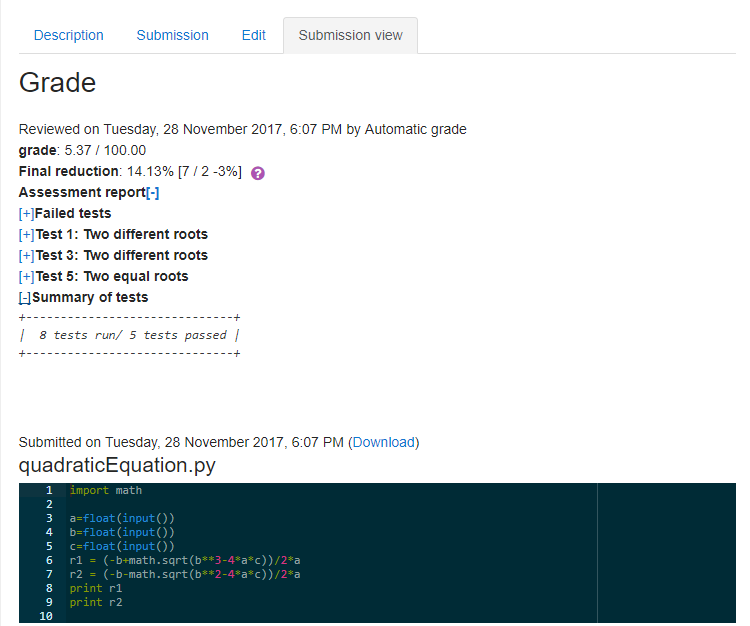
\includegraphics[]{moodle_vpl.png}
    }
    \caption{Moodle Virtual Programming Lab feladatbeadás}
    \label{fig:moodle_vpl}
\end{figure}

Elterjedtségének köszönhetően számos közösségi fejlesztésű modul is készült hozzá, melyek közül találhatunk szép számmal a programozás oktatására fókuszálókat is. Ilyen például a Virtual Programming Lab \cite{VPL} \cite{VPLJournal}, mely támogat forráskódszerkesztést a böngészőben, programok futtatását, ellenőrzését és plágium ellenőrzést is. Mindezt a felhasználók a már megszokott Moodle környezetben érhetik el a kényelmes használat érdekében.

\section{edX, Open edX}
Az edX \cite{EDXAbout} egy nonprofit online kezdeményezés, melynek alapítói a Harvard University és a Massachusetts Institute of Technology. Ennek segítségével egyetemi szintű kurzusokat tartanak világszerte közel 10 millió felhasználóval és több, mint ezer kurzussal \cite{EDXReview}.

Az edX rendszer nem csak egyszerű tananyagok megtekintésére biztosít lehetőséget, de videókat és egyéb feladatokat is találunk a kínált kurzusokban. Emellett egyszerűen kapcsolatba léphetünk másokkal, akik a kurzusunkat hallgatják, ha éppen segítségre lenne szükségünk. A kurzusok többnyire ingyenesek, de sok esetben van lehetőségünk fizetés ellenében igazolást kapnunk a sikeresen elvégzett kurzusról.

A portálon lehetőségünk van programozással kapcsolatos kurzusok felvételére is. Ezek keretében pedig online kód írásra, fordításra, futtatásra és a helyesség ellenőrzésére is van mód, amik nélkül az önálló tanulás nagyon nehézkes lenne. Webes kódolást némely kurzusnál Codeboard\footnotemark integrációval van megoldva, melynek köszönhetően nem is kell a tanuláshoz a megfelelő környezeteket telepítenünk a saját gépünkre.
\footnotetext{A Codeboard (http://codeboard.io) egy böngésző alapú fejlesztő környezet a programozás oktatás segítésére. Támogatja az edX, moodle, cursera és egyéb platformokat.}

Az Open edX egy nyílt forráskódú platform, melyet az edX fejlesztett ki és tett szabadon hozzáférhetővé saját oktatási környezetek létrehozására. Közel a teljes szerver oldali kód Python nyelven íródott, melynek széleskörű ismerttségének (és a rendszer nyílt forráskódú voltának) köszönhetően bárki kiegészítheti a meglévő kódot.

\section{Codeacademy}

A Codeacademy (\url{https://www.codecademy.com}) az előzőekhez haonlóan egy eLearning rendszer,mely felhasználói számára számos programnyelvhez kínál tanulási lehetőségeket, mint a Python, Java, PHP és JavaScript nyelvekhez. A weboldalon regisztráció után ingyenesen hozzáférhetünk a kurzusokhoz, de lehetőségünk van a Pro verziót is választani. Itt fizetés ellenében élő támogatást, tanulási egységenkénti ellenőrző kvízt és egyéb szolgáltatásokat kapunk. \cite{CodeacademyPro}

A tanulás során pár perces feladatokat kapunk. Ezek megoldását a böngészőben található fejlesztői környezet támogatja, azaz a böngészőben meg tudjuk írni és kipróbálni a kódunkat, megfelelőségéről pedig másodperceken belül értesülünk, látva mely tesztesetek futtotak le sikeresen és melyeknél volt probléma, ld. \ref{fig:codeacademy}. ábra.

\begin{figure}[h]
    \centering
    \resizebox{\textwidth}{!}{
        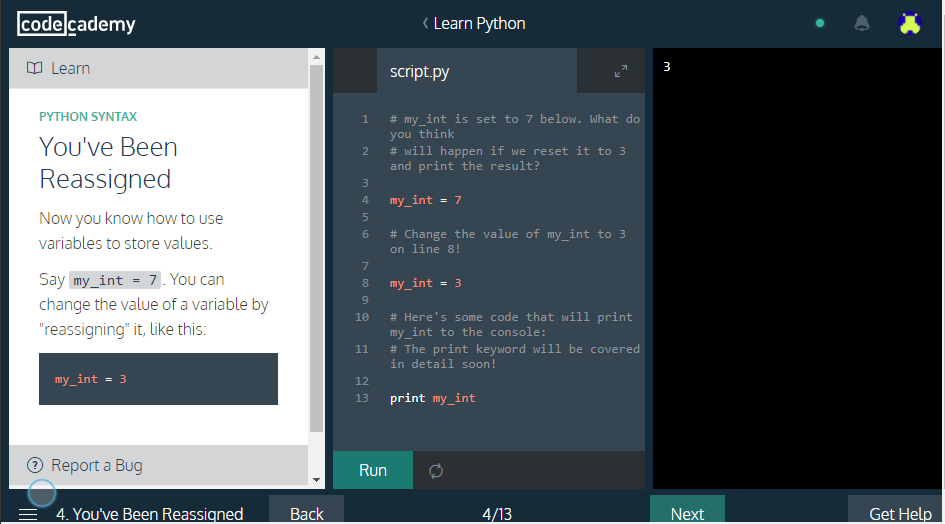
\includegraphics[]{codeacademy.png}
    }
    \caption[Codeacademy Python kurzus egyik feladata]{Codeacademy Python kurzus egyik feladata (forrás: \url{https://www.codecademy.com})}
    \label{fig:codeacademy}
\end{figure}

Az előzőleg felsoroltakkal szemben a Codeacademy nem nyílt forráskódú rendszer, így saját igényekre szabni nem lehet.

\section{Összefoglalás}

A felsorolt nyílt forráskódú rendszerek egy általános megoldást biztosítanak az internetes oktatásra. Ennek következtében a programozás specifikus feladatok létrehozása körülményesebb, illetve kevésbé személyre szabott lehet a létező moduloktól függően. Ezen okok adják a JPorta létjogosultságát, mivel az egy programozás orientált szemléletű, de mégis általános megoldást próbál nyújtani a felmerülő igényekre, melyeket a tervezési fázisban az oktatókkal közösen határozták meg.
%----------------------------------------------------------------------------
\chapter{A Jporta (5-10 oldal)}\label{chapter:jporta}
%----------------------------------------------------------------------------

Mi is a jporta, milyen funkciói vannak, gui...
%----------------------------------------------------------------------------
\chapter{Hallgatók értékelései}\label{chapter:assessments}
%----------------------------------------------------------------------------

\section{Értékelési rendszer (2-3 oldal)}
A korábban leírtaknak megfelelően a JPorta tárgyaiban lehetőség van különböző értékeléseket felvenni, majd azokat kurzusokhoz rendelni. Ezeket később a kurzus oktatói fogják értékelni.

Új értékelést csak a tárgy adminisztrátorai tudnak létrehozni és kurzusokhoz rendelni. Mindne értékeléshez az alábbi tulajdonságok tartoznak:
\begin{itemize}
    \item Név: rövid név, mely azonosítja az értékelést, pl. ZH 1
    \item Típus: előre definiált értékek, melyekhez tartozik egy reguláris kifejezés \cite{RegExp}. Csak olyan értéket vehet fel, ami illeszkedik a hozzá tartozó kifejezésre.
    \item Súly: meghatározza a sorrendet az értékelések megjelenítésénél.
    \item Ki értékelheti: kurzusokhoz, vagy csak a tárgyhoz rendelt oktatók értékelhetik.
    \item Dinamikus-e: az adott értékelés dinamikusan értékelődik-e ki, ld. \aref{section:dynamic-assessments} pontban.
    \item Privát-e: a privát értékeléseket csak az oktatók látják, a hallgatók nem.
    \item Megjegyzés: részletes leírása az értékelésnek, tipikusan dinamikus értékelések esetén hasznos.
    \item Kurzusok: tárgyon belül mely kurzusokhoz akarjuk hozzárendelni az értékelést.
\end{itemize}

\begin{figure}[h]
    \centering
    \resizebox{\textwidth}{!}{
        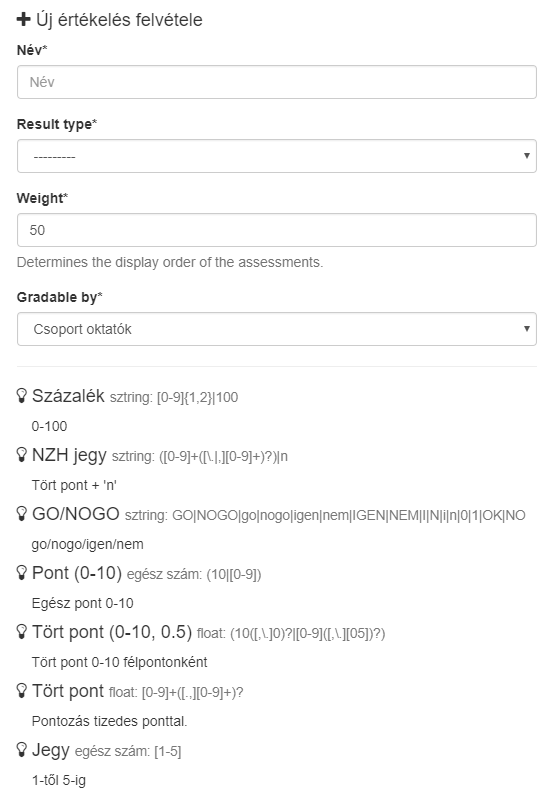
\includegraphics[]{jporta_add_result.png}
    }
    \caption{Értékelés típus hozzáadása}
    \label{fig:jporta_add_result}
\end{figure}

\begin{figure}[h]
    \centering
    \resizebox{\textwidth}{!}{
        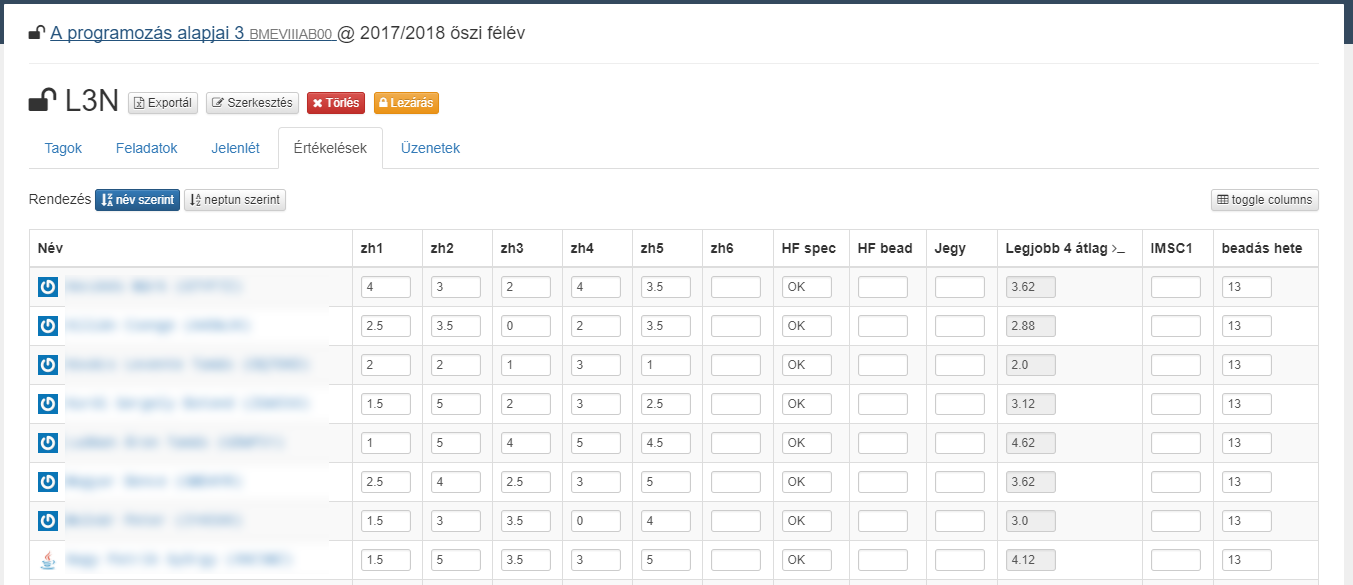
\includegraphics[]{jporta_course_results.png}
    }
    \caption{Hallgatók értékelései}
    \label{fig:jporta_course_results}
\end{figure}

\section{Dinamikus mezők (3-5 oldal)}\label{section:dynamic-assessments}

\subsection{Dinamikus mezők egymásra hivatkozása}
%----------------------------------------------------------------------------
\chapter{Automatizált feladatkiértékelő modul}\label{chapter:exercise}
%----------------------------------------------------------------------------

A JPorta egyik fő funkciója a beadott feladatmegoldások automatikus kiértékelése. Ennek tervezése során törekedtek az általános, könnyen bővíthető megoldás megtalálására, amikkel akár nem programozási jellegű feladatokat is ki lehet adni. \cite{DudiMsc}

Az elkészült modul blokkokat használ alapvető építő elemeinek, melyek egy-egy kiértékelési feladatot valósítanak meg. Ennek köszönhetően új igény esetén nem kell a meglévő blokkokat módosítani, csak az új funkciót megvalósító blokkot implementálni.

A blokkok közötti kommunikációt bemeneti és kimeneti csatlakozóik teszik lehetővé. Ezek szabadon összeköthetőek bármely más blokk ellenkező típusú csatlakozójával, pl. a felhasználói fájl blokk kimenetét ráköthetjük a GCC fordító blokk bemenetére, így lefordíhatjuk az adott forrásfájlt (blokkok típusait lásd lentebb). Ezen kívül lehetnek olyan paraméterei is egy blokknak, melyeket adminisztrátori felületen kell beállítani, pl. fordítás esetén a fordítónak átadott kapcsolók.

Ilyen meglévő blokkok a következők:

\begin{itemize}
    \item Specifikáció blokk: tartalmazza a feladat leírását, akár hallgató specifikus elemekkel (pl. neptun kód, név, egyedileg generált szám, stb.). 
    \item Szerzői fájl: a feladathoz oktatók által feltöltött fájlt tartalmazza. Szabályozható, hogy a felhasználók lássák-e ennek tartalmát. \label{authorfile}
    \item Felhasználói fájl blokk: hallgatói megoldásként feltöltött fájl.
    \item GCC fordító blokk: forrásfájlok fordítását végzi GCC fordítóval (\ref{fig:exercise_blokk}. ábra).
    \item Futtató blokk: futtatható fájlokat képes futtatni, kimeneteiket továbbítani.
    \item Szöveges ellenőrző blokk: bemenetén kapott szövegek összehasonlítását teszi lehetővé.
    \item Szkript ellenőrző blokk: különböző szkript nyelveken írt ellenőrzést tesz lehetővé, stb.
\end{itemize} 

\begin{figure}[p]
    \centering
    \resizebox{\textwidth}{!}{
        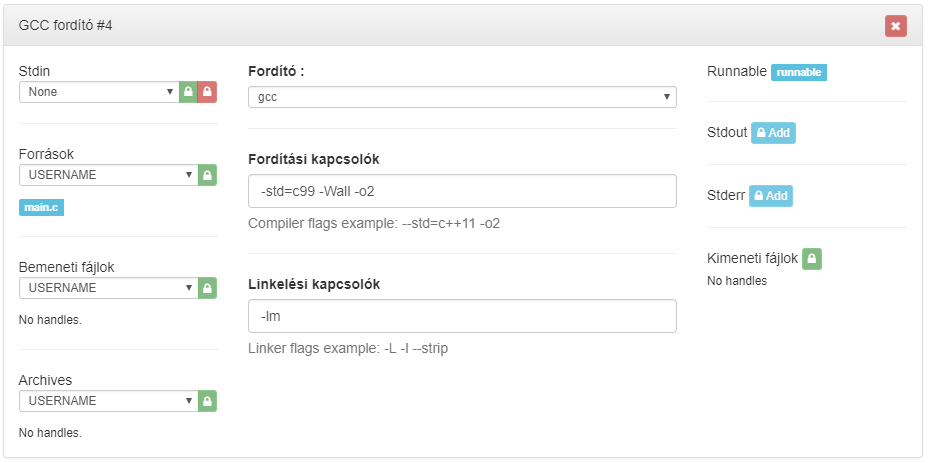
\includegraphics[]{exercise_blokk.png}
    }
    \caption{GCC fordító blokk adminisztrációs felülete}
    \label{fig:exercise_blokk}
\end{figure}

A beadás végső eredménye egy speciális blokk értéke lesz. Ennek a SubmissionResult blokknak egy bemente van, mely ha igaz a beadás sikeresnek tekinthető, ellenkező esetben sikertelen.

A blokkok kiértékelése (hasonlóan \aref{section:dynamic_dependencies}. pontban leírtakhoz) egy függőségi gráf felépítésével kezdődik, melynek kezdőpontja a fentebb említett SubmissionResult blokk. Csak azok a blokkok kerülnek kiértékelésre, amelyek (közvetve vagy közvetlen) függnek ettől a blokktól, hiszen a többi nem befolyásolja a beadás sikerességét.  Itt sem megengedettek a körkörös függőségek, tehát az elkészült gráfnak körmentesnek kell lennie.

\section{Jogosultságkezelés a JPortában}\label{subsection:permissions}

A JPorta által használt Django keretrendszer beépítetten tartalmaz egy egyszerű jogosultság kezelő rendszert. Ez lehetővé teszi különböző jogosultságok hozzárendelését felhasználókhoz, vagy felhasználói csoportokhoz. Minden Django modellhez \cite{DjangoModel} tartozik alapértelmezés szerint három jogosultság, melyeket a keretrendszer automatikusan hoz létre. Ezek a létrehozás (add), módosítás (change) és törlés (delete) jogosultságok. Sok esetben már ezek is elegek lehetnek számunkra, de bármikor létrehozhatunk új jogosultságokat, melyekkel személyre szabottabban tudjuk kezelni a hozzáférést egy-egy funkcióhoz. Ezeknek köszönhetően alapvteően egyszerűen kezelhetjük a jogosultságok kérdését \cite{DjangoAuth}. Fontos megjegyezni, hoyg Django-ban a \textit{superuser}-nek jelölt felhasználók automatikusan rendelkeznek minden jogosultsággal.

A JPorta ezen felül egyedi megoldást alkalmaz az egyes objektum példányok elérésének szabályozására, mely az access control list (ACL, \cite{ACL}) technikához hasonló. Az ACL minden objektumhoz rendel egy mátrixot, mely oszlopaiban a személyek (actor), soraiban pedig az egyes műveletek (action) találhatóak. Egy személy akkor hajthat végre egy műveletet, ha a mátrix általa és a művelet által meghatározott cellája igaz értéket tartalmaz.

\Aref{fig:acl}. ábra egy ilyen példát szemléltet: az objektumhoz tartozó hozzáférési mátrix értelmében Bob-nak csak olvasási, Alice-nak pedig olvasási és írási joga van. Emiatt Alice mind az olvasási, mind az írási műveletet sikeresen végrehajthatja, Bob azonban írási műveletet nem hajthat végre.

\begin{figure}[h]
    \centering
    \resizebox{\textwidth}{!}{
        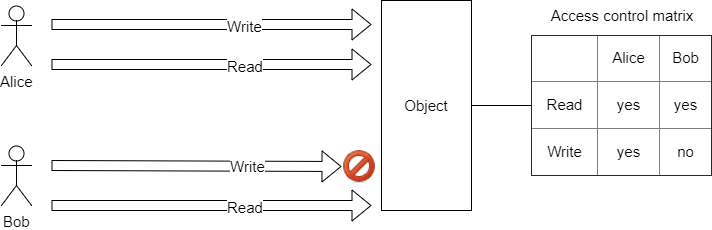
\includegraphics[]{ACL.png}
    }
    \caption{ACL működése és egy hozzáférési mátrix}
    \label{fig:acl}
\end{figure}

A portál közvetlen jogosultságok helyett jogosultsági szinteket használ, tipikusan tulajdonosi (owner) és operátori (operator) szintekkel, de ez modellenként eltérő lehet. Ilyenkor ha egy felhasználót egy objektum tulajdonosának jelölünk, egyben operátori jogosultságokkal is felruházzuk. Ha egy felhasználónak nem kívánunk jogosultságot adni az adott objektumhoz, akkor nem jelöljük egyik szinten sem. Fontos megjegyezni, hogy a \textit{superuser}-nek jelölt felhasználók itt is automatikusan rendelkeznek minden jogosultsági szinttel.

Ez a megoldás kifinomultabbnak mondható az eredeti ACL technikához képest, mivel így különböző műveletek halmazát rendelhetjük egy adott szinthez, pl. az operátor jogosult megtekinteni és módosítani az adott objektum tulajdonságait, de a törléshez már tulajdonosi szintre van szükség.

\section{Jogosultságkezelés felülvizsgálata}

Az automatikus kiértékelő modulnál a jogosultság kezelés korábban nem készült el megfelelően, így ugyan hallgatói oldalról nézve minden jól működött, a feladatokat csak \textit{superuser} jogokkal rendelkező adminisztrátorok hozhatták létre. Ez pedig nagyban megnehezítette felsőbbéves hallgatók, laborvezetők bevonását a rendelkezésre álló feladatok bővítésére. Ennek oka, hogy ekkor minden más adatot is láttak volna a portálon, beleértve minden hallgató eredményeit, megoldásait, ami nem megengedhető.

Ezek értelmében a jogosultság kezelés kibővítésével a cél az volt, hogy egyszerűen és biztonságosan lehessen automatikusan kiértékelődő feladatok létrehozására és szerkesztésére. Az így elkészült rendszer alkalmazza mindkét fenti hozzáférés szabályozási módszert a maximális biztonság és testreszabottság elérésének érdekében.

Ennek elkészítéséhez először a Django jogosultságok ellenőrzését implementáltam, melyhez a beépített \textit{PermissionRequiredMixin} osztályt használtam. Ez egyszerűen teszi lehetővé a jogosultságok meglétének ellenőrzését, csak meg kell adnunk a szükséges jogosultság(ok) listáját, a többit pedig a keretrendszerre bízhatjuk. \cite{DjangoPermissionMixin}

Két jogosultságot használtam fel:

\begin{itemize}
    \item \textit{view\_exercise}: meglétével a felhasználó megtekintheti az összes eddig létrehozott automatikusan kiértékelődő feladatot (exercise). Ennek köszönhetően láthatja, ha már létezik hasonló feladat, mint amire szüksége van, illetve ötletet meríthet a többi feladatból. Emellett pedig a tanulási folyamatot is segíti, hiszen a már meglévő feladatok megértésével fény derülhet az addig rejtélyesnek tűnő működésre.
    \item \textit{create\_exercise}: meglétével a felhasználó létrehozhat új feladatokat. Ilyenkor lehetősége van új, üres feladatot létrehozni vagy egy korábbiról másolatot készíteni.
\end{itemize}

Ezek a jogosultságok fedik le általánosságban a hozzáférések szabályozását. A konkrét feladat példányok hozzáférésének konrtollálásához az előzőek kiegészítésére operátori és tulajdonosi szintet használtam. Ha egy felhasználóhoz egyik sincs hozzárendelve, akkor csak megtekintheti az adott feladatot, nem módosíthatja annak semmilyen elemét. A felhasználói szintek beállítása \aref{fig:exercise_perms}. ábrán látható.

\begin{itemize}
    \item Operátor (operator): az adott feladat példány alap adatait (cím, leírás és címkék), meglévő blokkjait, azok összeköttetéseit tudja módosítani. Lehetősége van más operátor szintű felhasználók felvételére is, illetve egy beadott feladatra újra lefuttatni a kiértékelési folyamatot.
    \item Tulajdonos (owner): az adott feladat példányhoz teljes jogkörrel rendelkezik. Az operátori szint jogain felül hozzáadhat, törölhet blokkokat, más személyeket tulajdonosi szintre emelhet és akár törölheti is a feladatot. Csak tulajdonosok publikálhatnak vagy vonhatnak vissza feladatokat\footnote{A feladat publikálása késznek jelöli azt, melyet csak ilyen állapotban lehet kurzushoz rendelni.}.
\end{itemize}

\begin{figure}[h]
    \centering
    \resizebox{\textwidth}{!}{
        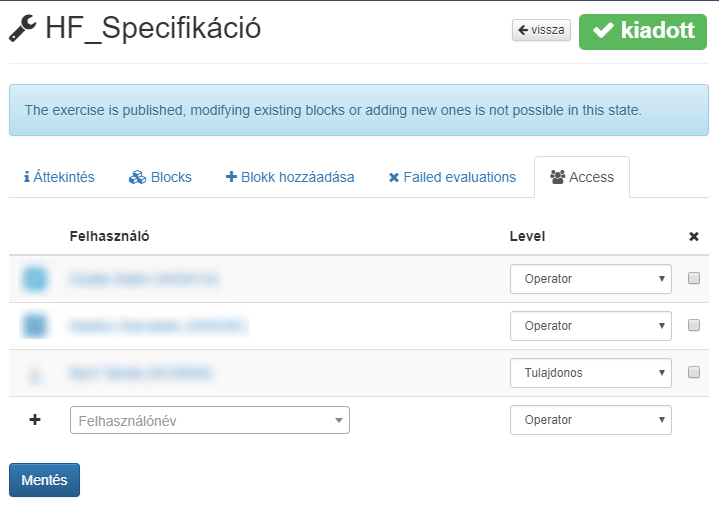
\includegraphics[]{exercise_perms.png}
    }
    \caption{Feladat példányhoz tartozó jogosultsági szintek beállítása}
    \label{fig:exercise_perms}
\end{figure}

Végezetül a szerzői fájlok (ld. \aref{chapter:exercise}. fejezet) hozzáférését ellenőriztem. Itt van lehetőségünk a hallgatók elől elrejteni az adott fájlt, ugyanakkor ez csak a feladatbeadásnál való listázottságát módosítja csak. A fájlok webcím alapján közvetlenül továbbra is elérhetőek maradtak, így próbálgatással az összes titkosnak hitt szerzői fájl tartarlmát le lehetett kérdezni. Ennek megoldása egyszerűnek bizonyult, csak módosítani kellett a kérést kezelő függvényben a felhasználó és a visszaadandó fájl ellenőrzését. Eddig a fájl titkos voltától függetlenül visszaadásra került a tartalom.

\section{Kód lefedettség ellenőrzés}

\section{Feladatok (tesztek) importálása és exportálása}

\section{Feladatok csoportosítása}

\section{További lehetőségek}

\subsection{Plágiumkeresés}

\subsection{Verziókezelő támogatás}
%----------------------------------------------------------------------------
\chapter*{Összefoglalás}\addcontentsline{toc}{chapter}{Összefoglalás}
%----------------------------------------------------------------------------

A szakdolgozatom keretében részletesen megismertem mind a JPorta rendszerét, mind a felé támasztott elvárásokat oktatói és hallgatói szempontból. Ezek alapján főként az aktuálisan legkritikusabbnak ítélt területek fejlesztésével foglalkoztam, azaz a dinamikus mezőkkel és az automatikusan kiértékelődő feladatok rendszerével.

Előbbin elért eredményeknek köszönhetően az oktatók már létrehozhatnak olyan dinamikus értékelési mezőket, melyek más dinamikus mezőket is használnak a számításaik során. Ezzel segítik az oktatókat a bonyolultabb mezők elkészítésében. Tipikusan ez a félév végi eredmény meghatározásánál lehet különösen hasznos.

Az automatikus kiértékelő rendszer fejlesztésének köszönhetően már lehetőség van oktatóknak és hallgatóknak is jogosultságot adni a feladatok létrehozására. Ez egy további lépést jelent a tárgyak széleskörű támogatására, hiszen így a feladatok elkészítésére nem csak a portál adminisztrátorait lehet megkérni, hanem minden arra jogosult személy kísérletezhet.

A kódlefedettség ellenőrző pedig lehetőséget teremt a C és C++ nyelvű feladatok esetén a tesztesetek értékelésére. Így könnyebb automatikusan kiszűrni a hibákat, működési zavarokat a beadott megoldásokban.

Végezetül pedig további hasznos funkciókra tettem javaslatot, melyek tovább növelhetik az oktatók és hallgatók elégedettségét a portállal szemben.
%----------------------------------------------------------------------------
\chapter*{Köszönetnyilvánítás}\addcontentsline{toc}{chapter}{Köszönetnyilvánítás}
%----------------------------------------------------------------------------

Szerenték köszönetet mondani konzulensemnek, Dr.~Szeberényi Imrének, aki a tanulmányaim és szakdolgozatom készítésének során végig támogatott.

Emellett külön köszönet jár a BME Informatikai Központ munkatársainak és volt munkatársainak, köztük Dudás Ádámnak és Kálmán Viktornak, akik a korábbi években elkészítették a JPorta fő moduljait és ezekkel kapcsolatban a félév során hasznos információkkal segítették munkámat.
\listoffigures\addcontentsline{toc}{chapter}{Ábrák jegyzéke}
%\listoftables\addcontentsline{toc}{chapter}{Táblázatok jegyzéke}
%\printglossary[title=Rövidítések jegyzéke]

\bibliography{bibliography}\addcontentsline{toc}{chapter}{Irodalomjegyzék}
\bibliographystyle{huplain}

\label{page:last}
\end{document}
